
\documentclass[10pt]{beamer}
\usetheme{metropolis}

% ── Packages ──
\usepackage{amsmath,amssymb,amsthm}
\usepackage{tikz}
\usetikzlibrary{positioning,arrows.meta,fit,matrix,backgrounds,calc,shapes.geometric,decorations.pathreplacing,angles,quotes}
\usepackage{graphicx}
\usepackage{array}
\usepackage{etoolbox}
\usepackage{cancel}

% ── Theorem environments ──
\theoremstyle{definition}
\newtheorem{defi}{Definition}[section]
\newtheorem{prop}{Proposition}[section]
\newtheorem{thm}{Theorem}[section]
\newtheorem{cor}{Corollary}[section]

% Custom theorem styles with colors
\setbeamercolor{block title}{bg=red!75!black,fg=white}
\setbeamercolor{block body}{bg=yellow!10!white}

\AtBeginEnvironment{prop}{%
  \setbeamercolor{block title}{bg=yellow!75!black,fg=black}%
  \setbeamercolor{block body}{bg=yellow!10!white}%
}
\AtEndEnvironment{prop}{%
  \setbeamercolor{block title}{bg=red!75!black,fg=white}%
}

\AtBeginEnvironment{thm}{%
  \setbeamercolor{block title}{bg=yellow!75!black,fg=black}%
  \setbeamercolor{block body}{bg=yellow!10!white}%
}
\AtEndEnvironment{thm}{%
  \setbeamercolor{block title}{bg=red!75!black,fg=white}%
}

\AtBeginEnvironment{cor}{%
  \setbeamercolor{block title}{bg=yellow!75!black,fg=black}%
  \setbeamercolor{block body}{bg=yellow!10!white}%
}
\AtEndEnvironment{cor}{%
  \setbeamercolor{block title}{bg=red!75!black,fg=white}%
}

% ── Highlighting ──
\newcommand{\x}[1]{\alert{\textbf{#1}}}

% ── Color shortcuts ──
\newcommand{\rd}[1]{{\color{red!70!black}#1}}
\newcommand{\bl}[1]{{\color{blue!70!black}#1}}
\newcommand{\gn}[1]{{\color{green!60!black}#1}}

\title{Lecture 17: Complex Numbers}
\subtitle{MATH203 Applied Linear Algebra}
\date{}
\titlegraphic{}

\begin{document}
\maketitle


% ┌─────────────────────────────────────────────────────────────────────┐
% │ SECTION 1: OUR MACHINERY BREAKS OVER R                            │
% │                                                                    │
% │ THE MACRO DESIGN: START FROM THE GAP IN L14–L16                   │
% │                                                                    │
% │ The audience enters having built a powerful pipeline:               │
% │   det(tI-A) → factor → eigenvalues → spectral projections →       │
% │   value tables → diagonalization.                                  │
% │ But this pipeline relied on an assumption: the minimal polynomial  │
% │ factors into distinct linear factors.                              │
% │                                                                    │
% │ This section makes them FEEL the gap. The rotation matrix is       │
% │ geometrically obvious (everyone knows what 90° rotation does)      │
% │ but the pipeline can't touch it. The emotional beat:               │
% │   Frame 1: "remember our pipeline" (comfort)                      │
% │   Frame 2: "two restrictions remain" (awareness)                  │
% │   Frame 3-4: "rotation matrix breaks it" (tension)                │
% │   Frame 5-6: "can we fix it?" → "yes" (resolution promised)      │
% │                                                                    │
% │ Key pedagogical choice: state BOTH restrictions up front.          │
% │ Complex numbers fix (a) but NOT (b). This honesty prevents the    │
% │ false impression that C solves everything. JCF handles (b) and    │
% │ is flagged as self-study.                                          │
% └─────────────────────────────────────────────────────────────────────┘
\section{Our Machinery Breaks Over $\mathbb{R}$}


\begin{frame}{Recall: The Pipeline from L14--L16}

In Lectures 14--16, we built a powerful pipeline:

\vfill

\begin{center}
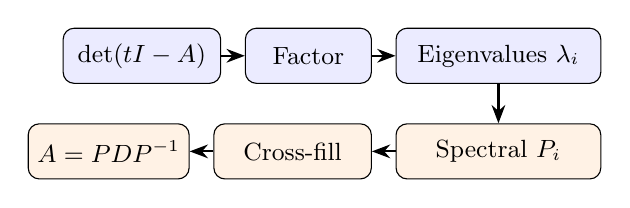
\begin{tikzpicture}[>=Stealth, node distance=0.3cm, every node/.style={font=\small}]
  \node[draw, rounded corners, fill=blue!8, minimum width=2.0cm, minimum height=0.7cm] (det) {$\det(tI - A)$};
  \node[right=of det, draw, rounded corners, fill=blue!8, minimum width=1.6cm, minimum height=0.7cm] (fac) {Factor};
  \node[right=of fac, draw, rounded corners, fill=blue!8, minimum width=2.6cm, minimum height=0.7cm] (eig) {Eigenvalues $\lambda_i$};

  \node[below=0.5cm of eig, draw, rounded corners, fill=orange!10, minimum width=2.6cm, minimum height=0.7cm] (spec) {Spectral $P_i$};
  \node[left=of spec, draw, rounded corners, fill=orange!10, minimum width=2.0cm, minimum height=0.7cm] (cross) {Cross-fill};
  \node[left=of cross, draw, rounded corners, fill=orange!10, minimum width=2.0cm, minimum height=0.7cm] (diag) {$A = PDP^{-1}$};

  \draw[->, thick] (det) -- (fac);
  \draw[->, thick] (fac) -- (eig);
  \draw[->, thick] (eig) -- (spec);
  \draw[->, thick] (spec) -- (cross);
  \draw[->, thick] (cross) -- (diag);
\end{tikzpicture}
\end{center}

\vfill

This works when the minimal polynomial factors into \x{distinct linear factors}.

\vfill\pause

But there are \x{two restrictions} in this assumption:

\begin{enumerate}
\item[(a)] The polynomial must factor into \x{linear} factors.
\item[(b)] Those factors must be \x{distinct} (no repeated roots in the minimal polynomial).
\end{enumerate}

\end{frame}


\begin{frame}{Today and Beyond}

\begin{center}
\renewcommand{\arraystretch}{1.5}
{\small
\begin{tabular}{p{3.2cm}|p{3.0cm}|p{3.0cm}}
Restriction & Problem & Solution \\
\hline
\x{(a)} Cannot factor into linear factors over $\mathbb{R}$ & Some polynomials are irreducible over $\mathbb{R}$ & \x{Today:} Complex numbers $\mathbb{C}$ \\
\hline
(b) Repeated factors in the minimal polynomial & Lagrange interpolation fails: observation points collapse, losing information & Self-study: Jordan Canonical Form
\end{tabular}
}
\end{center}

\vfill\pause

Today we address \x{restriction (a)} only.

\vfill

Restriction (b) requires completely different tools (Jordan Canonical Form) --- this will be \x{self-study material}.

\vfill

Complex numbers do \x{not} solve restriction (b).

\end{frame}


% ADR: The rotation matrix is the perfect example because:
% (1) Everyone can visualize 90° rotation -- no abstraction needed.
% (2) det(tI - R) = t^2 + 1 is the simplest irreducible polynomial over R.
% (3) The emotional contrast: "I know exactly what this matrix does,
%     but the pipeline can't even start" is powerful.
\begin{frame}[shrink=5]{The Pipeline Breaks: A Concrete Example}

The \x{90\textdegree{} rotation matrix}:

$$R = \begin{pmatrix} 0 & -1 \\ 1 & 0 \end{pmatrix}$$

\vfill

\begin{columns}
\column{0.45\textwidth}
\begin{center}
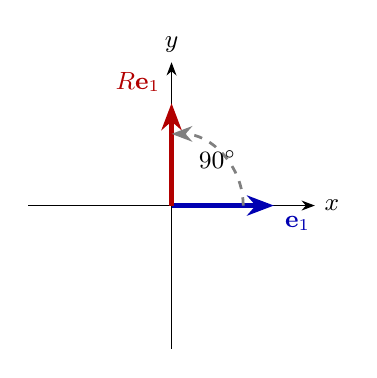
\begin{tikzpicture}[>=Stealth, scale=1.3]
  \draw[->] (-1.4,0) -- (1.4,0) node[right] {\small $x$};
  \draw[->] (0,-1.4) -- (0,1.4) node[above] {\small $y$};
  \draw[->, blue!70!black, line width=1.5pt] (0,0) -- (1,0) node[below right] {\small $\mathbf{e}_1$};
  \draw[->, red!70!black, line width=1.5pt] (0,0) -- (0,1) node[above left] {\small $R\mathbf{e}_1$};
  \draw[->, gray, dashed, line width=1pt] (0.7,0) arc[start angle=0, end angle=90, radius=0.7];
  \node at (0.45,0.45) {\small $90^{\circ}$};
\end{tikzpicture}
\end{center}

\column{0.55\textwidth}

We know \x{exactly} what $R$ does: it rotates every vector by $90^{\circ}$ counterclockwise.

\vfill

Geometrically clear. No mystery.

\end{columns}

\vfill\pause

Compute the characteristic polynomial:

$$\det(tI - R) = \det\begin{pmatrix} t & 1 \\ -1 & t \end{pmatrix} = t^2 + 1$$

\end{frame}


\begin{frame}{The Pipeline Stops}

$$\det(tI - R) = t^2 + 1$$

\vfill

$t^2 + 1$ has \x{no real roots}.

\vfill

It does \x{not} factor into linear factors over $\mathbb{R}$.

\vfill\pause

\begin{center}
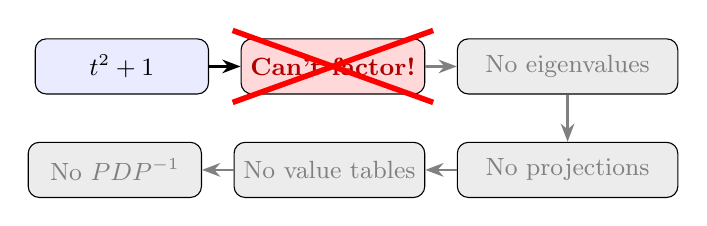
\begin{tikzpicture}[>=Stealth, node distance=0.4cm, every node/.style={font=\small}]
  \node[draw, rounded corners, fill=blue!8, minimum width=2.2cm, minimum height=0.7cm] (det) {$t^2 + 1$};
  \node[right=of det, draw, rounded corners, fill=red!15, minimum width=2.2cm, minimum height=0.7cm, text=red!70!black] (fac) {\textbf{Can't factor!}};
  \node[right=of fac, draw, rounded corners, fill=gray!15, minimum width=2.8cm, minimum height=0.7cm, text=gray] (eig) {No eigenvalues};

  \node[below=0.6cm of eig, draw, rounded corners, fill=gray!15, minimum width=2.8cm, minimum height=0.7cm, text=gray] (spec) {No projections};
  \node[left=of spec, draw, rounded corners, fill=gray!15, minimum width=2.2cm, minimum height=0.7cm, text=gray] (val) {No value tables};
  \node[left=of val, draw, rounded corners, fill=gray!15, minimum width=2.2cm, minimum height=0.7cm, text=gray] (diag) {No $PDP^{-1}$};

  \draw[->, thick] (det) -- (fac);
  \draw[->, thick, gray] (fac) -- (eig);
  \draw[->, thick, gray] (eig) -- (spec);
  \draw[->, thick, gray] (spec) -- (val);
  \draw[->, thick, gray] (val) -- (diag);

  \draw[red, line width=2pt] ($(fac.north west)+(-0.1,0.1)$) -- ($(fac.south east)+(0.1,-0.1)$);
  \draw[red, line width=2pt] ($(fac.north east)+(0.1,0.1)$) -- ($(fac.south west)+(-0.1,-0.1)$);
\end{tikzpicture}
\end{center}

\vfill

The matrix $R$ is \x{perfectly concrete} --- it rotates by $90^{\circ}$.

\vfill

The problem is not the matrix. The problem is the \x{number system}.

\end{frame}


\begin{frame}{The Question}

Can we extend $\mathbb{R}$ to a \x{larger number system} where $t^2 + 1 = 0$ \x{has} solutions?

\vfill\pause

And not just for this one polynomial --- does \x{every} polynomial factor into linear factors there?

\vfill\pause

\begin{block}{Spoiler: Fundamental Theorem of Algebra}
Over the \x{complex numbers} $\mathbb{C}$, every degree-$n$ polynomial has exactly $n$ roots (counted with multiplicity).

\vfill

$$p(t) = (t - z_1)(t - z_2)\cdots(t - z_n), \qquad z_i \in \mathbb{C}$$

\vfill

\x{Every} polynomial factors into linear factors. Restriction (a) is completely removed.
\end{block}

\end{frame}


% ┌─────────────────────────────────────────────────────────────────────┐
% │ SECTION 2: THE CUBIC FORMULA — COMPLEX NUMBERS ARE UNAVOIDABLE    │
% │                                                                    │
% │ THE MACRO DESIGN: HISTORICAL INEVITABILITY                        │
% │                                                                    │
% │ The audience might think: "ok, so you just DEFINED sqrt(-1) to    │
% │ exist. That feels like cheating." This section counters that       │
% │ reaction with the historical fact: even for REAL problems with    │
% │ REAL answers, the solution path forces you through sqrt(-1).      │
% │                                                                    │
% │ The cubic formula is the key example. The emotional arc:           │
% │   Frame 1: "quadratic formula — easy to dismiss sqrt(-1)" (setup) │
% │   Frame 2: "cubic formula exists, it's monstrous" (curiosity)    │
% │   Frame 3: "use it on x^3=x... get sqrt(-1)???" (shock)          │
% │   Frame 4: "Bombelli: compute with it, get real answers" (awe)   │
% │   Frame 5: "you cannot avoid it" (conviction)                    │
% │                                                                    │
% │ This section also serves as a physics/applied motivation:          │
% │ waves, quantum mechanics, electrical engineering all require C.   │
% │ Even when the problem is entirely real, the solution uses C.      │
% └─────────────────────────────────────────────────────────────────────┘
\section{The Cubic Formula: Complex Numbers Are Unavoidable}


\begin{frame}{The Quadratic Formula}

For $ax^2 + bx + c = 0$:

$$x = \frac{-b \pm \sqrt{b^2 - 4ac}}{2a}$$

\vfill

When $b^2 - 4ac < 0$: ``no real solutions.''

\vfill\pause

Easy to dismiss $\sqrt{-1}$ --- just say ``no solution'' and move on.

\vfill

But what about \x{cubic} equations?

\end{frame}


\begin{frame}[shrink=5]{The Cubic Equation}

\begin{columns}
\column{0.65\textwidth}

$$ax^3 + bx^2 + cx + d = 0$$

\vfill

Unsolved for centuries --- until \x{1530}.

\vfill

Scipione del Ferro found a method, kept it secret until his deathbed. His student Antonio Fior learned it. Eventually Cardano published the formula.

\vfill\pause

Why doesn't your teacher show you this formula?

\column{0.3\textwidth}
\begin{center}
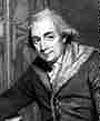
\includegraphics[width=\textwidth]{Pictures/cubic.jpg}
\end{center}
\end{columns}

\vfill\pause

Because it looks like this:

\[
\scalebox{0.78}{$\displaystyle\boxed{x = \sqrt[3]{\left(-\frac{b^3}{27a^2}+\frac{bc}{6a^2}-\frac{d}{2a}\right)+\sqrt{\Delta}}+\sqrt[3]{\left(-\frac{b^3}{27a^2}+\frac{bc}{6a^2}-\frac{d}{2a}\right)-\sqrt{\Delta}}-\frac{b}{3a}}$}
\]

\vfill

where $\Delta = \left(-\frac{b^3}{27a^2}+\frac{bc}{6a^2}-\frac{d}{2a}\right)^2+\left(\frac{c}{3a}-\frac{b^2}{9a^2}\right)^3$.

\end{frame}


\begin{frame}{The Paradox}

Use the cubic formula on a simple equation:

$$x^3 = x$$

\vfill

Obviously the solutions are $x = 0, \; 1, \; -1$.

\vfill\pause

But the cubic formula gives:

$$x = \frac{1}{\sqrt{3}}\left(\sqrt[3]{\sqrt{-1}} + \sqrt[3]{-\sqrt{-1}}\right)$$

\vfill\pause

This looks \x{insane}. There is a $\sqrt{-1}$ inside a cube root!

\vfill

And yet... if you compute with $\sqrt{-1}$ formally, you get back $0, \; 1, \; -1$.

\end{frame}


\begin{frame}{Bombelli's Insight (1572)}

Rafael Bombelli was the first to take $\sqrt{-1}$ seriously.

\vfill

His discovery: if you \x{compute with $\sqrt{-1}$ formally} --- treating it as an algebraic symbol with $(\sqrt{-1})^2 = -1$ --- the cubic formula \x{works}.

\vfill\pause

$\sqrt{-1}$ appears in the \x{middle} of the calculation...

\vfill

...but \x{cancels out} at the end, giving real answers.

\vfill\pause

For centuries, mathematicians had assumed $\sqrt{-1}$ ``does not exist.''

\vfill

But this assumption \x{blocked} them from using a perfectly valid formula.

\vfill

\x{You cannot assume $\sqrt{-1}$ does not exist. It is meaningful and must be computed.}

\end{frame}


\begin{frame}{The Lesson}

\begin{block}{Complex numbers are not optional}
Even when the \x{problem} involves only real numbers and the \x{answer} is real, the \x{solution path} may force you through $\sqrt{-1}$.

\vfill

This is not a trick or a convenience --- it is a \x{mathematical necessity}.
\end{block}

\vfill\pause

This pattern appears throughout science:

\vfill

\begin{itemize}
\item \x{Waves:} oscillations naturally described by $e^{i\theta}$
\item \x{Quantum mechanics:} the Schr\"odinger equation lives in $\mathbb{C}$
\item \x{Electrical engineering:} impedance uses complex arithmetic
\end{itemize}

\vfill

Even when the physical measurement is real, the \x{mathematics behind it} uses complex numbers.

\end{frame}


% ┌─────────────────────────────────────────────────────────────────────┐
% │ SECTION 3: DEFINITION & THE COMPLEX PLANE                         │
% │                                                                    │
% │ THE MACRO DESIGN: GROUND THE ABSTRACTION IN GEOMETRY              │
% │                                                                    │
% │ Now the audience is motivated: they NEED complex numbers.          │
% �� This section gives the formal definition, immediately grounded    │
% │ in the complex plane (R^2 with multiplication).                   │
% │                                                                    │
% │ Key choice: addition first (familiar — same as vector addition).   │
% │ Multiplication comes in the NEXT section as the deep surprise.    │
% │                                                                    │
% │ Legacy source: MANR.tex lines 1–37.                               │
% │ TikZ diagrams adapted from the legacy blue/red vector drawings.   │
% └─────────────────────────────────────────────────────────────────────┘
\section{The Complex Numbers}


\begin{frame}{Definition}

We write $i = \sqrt{-1}$, so that $i^2 = -1$.

\vfill

\begin{defi}
A \x{complex number} is a number of the form
$$z = a + bi, \qquad a, b \in \mathbb{R}$$
where $a$ is the \x{real part} and $b$ is the \x{imaginary part}.
\end{defi}

\vfill

The set of all complex numbers is denoted $\mathbb{C}$.

\vfill\pause

$$\underbrace{\mathbb{N}}_{\text{natural}} \;\subset\; \underbrace{\mathbb{Z}}_{\text{integer}} \;\subset\; \underbrace{\mathbb{Q}}_{\text{rational}} \;\subset\; \underbrace{\mathbb{R}}_{\text{real}} \;\subset\; \underbrace{\mathbb{C}}_{\text{complex}}$$

\end{frame}


\begin{frame}[shrink=3]{The Complex Plane}

A complex number $a + bi$ corresponds to a point $(a, b)$ in $\mathbb{R}^2$.

\vfill

\begin{center}
\begin{tikzpicture}[>=Stealth, scale=1.2]
  \draw[->] (-2.5,0) -- (2.5,0) node[right] {$\mathbb{R}$};
  \draw[->] (0,-1.5) -- (0,2.5) node[above] {$i\mathbb{R}$};

  \draw[ultra thick, red!70!black, ->] (0,0) -- (1,2) node[above right] {$1 + 2i$};
  \draw[thick, dotted, gray] (1,2) -- (1,0) node[below] {\small $1$};
  \draw[thick, dotted, gray] (1,2) -- (0,2) node[left] {\small $2i$};

  \fill (0,0) circle (2pt);
  \foreach \x in {-2,-1,1,2} {\draw (\x,0.05) -- (\x,-0.05) node[below, font=\tiny] {$\x$};}
  \foreach \y in {-1,1,2} {\draw (0.05,\y) -- (-0.05,\y);}
\end{tikzpicture}
\end{center}

\vfill

The horizontal axis is the \x{real axis} ($\mathbb{R}$).

The vertical axis is the \x{imaginary axis} ($i\mathbb{R}$).

\end{frame}


\begin{frame}{Addition = Parallelogram Law}

$$(a + bi) + (c + di) = (a + c) + (b + d)i$$

\vfill

Addition of complex numbers is \x{the same as vector addition in $\mathbb{R}^2$}.

\vfill

\begin{center}
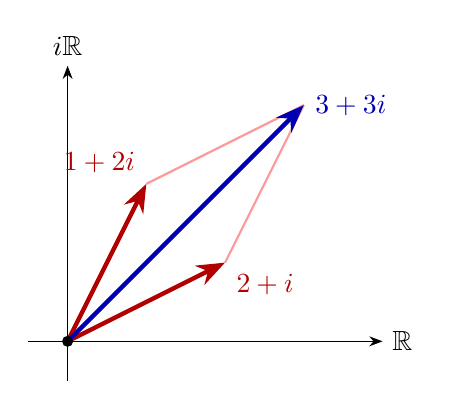
\begin{tikzpicture}[>=Stealth, scale=1.0]
  \draw[->] (-0.5,0) -- (4,0) node[right] {$\mathbb{R}$};
  \draw[->] (0,-0.5) -- (0,3.5) node[above] {$i\mathbb{R}$};

  \draw[ultra thick, red!70!black, ->] (0,0) -- (1,2) node[above left] {$1 + 2i$};
  \draw[ultra thick, red!70!black, ->] (0,0) -- (2,1) node[below right] {$2 + i$};

  \draw[thick, red!40] (1,2) -- (3,3);
  \draw[thick, red!40] (2,1) -- (3,3);

  \draw[ultra thick, blue!70!black, ->] (0,0) -- (3,3) node[right] {$3 + 3i$};

  \fill (0,0) circle (2pt);
\end{tikzpicture}
\end{center}

\vfill

$(1+2i) + (2+i) = 3 + 3i$

\end{frame}


\begin{frame}{Multiplication: The Surprise}

Addition is familiar --- same as vectors.

\vfill

But complex numbers can be \x{multiplied}, and this is where the magic happens.

\vfill\pause

To multiply, expand as a polynomial in $i$ and use $i^2 = -1$:

$$(3 + i)(5 + i) = 15 + 3i + 5i + \underbrace{i^2}_{= -1} = 14 + 8i$$

\vfill\pause

In general:

$$(a + bi)(c + di) = \underbrace{(ac - bd)}_{\text{real part}} + \underbrace{(ad + bc)}_{\text{imaginary part}} \cdot i$$

\vfill

\x{Next section:} What does multiplication \x{look like} geometrically?

\end{frame}


% ┌─────────────────────────────────────────────────────────────────────┐
% │ SECTION 4: MULTIPLICATION = ROTATION + SCALING                     │
% │                                                                    │
% │ THE MACRO DESIGN: GEOMETRY OF MULTIPLICATION                      │
% │                                                                    │
% │ This is the CORE visual section. The audience sees that            ���
% │ multiplication by i is 90° rotation (connecting back to the       │
% │ rotation matrix from §1!), and general multiplication is          │
% │ rotation + scaling.                                                │
% │                                                                    │
% │ Legacy source: MANR.tex lines 38–201 (blue→red square TikZ).     │
% │ The blue-square-to-red-square animation is the key visual.        │
% └─────────────────────────────────────────────────────────────────────┘
\section{Multiplication = Rotation + Scaling}


\begin{frame}[shrink=5]{Multiplying by $i$}

Since $i^2 = -1$:
$$i \cdot (a + bi) = -b + ai$$

\vfill

\begin{columns}
\column{0.5\textwidth}
\begin{center}
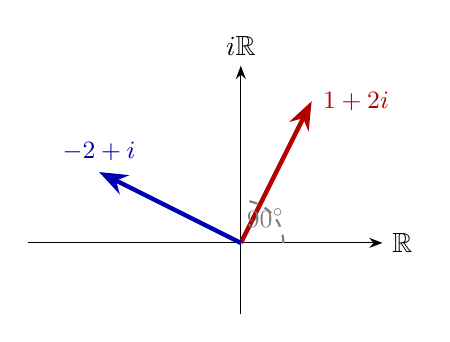
\begin{tikzpicture}[>=Stealth, scale=0.9]
  \draw[->] (-3.0,0) -- (2.0,0) node[right] {$\mathbb{R}$};
  \draw[->] (0,-1.0) -- (0,2.5) node[above] {$i\mathbb{R}$};

  \draw[ultra thick, red!70!black, ->] (0,0) coordinate (O) -- (1,2) coordinate (A) node[right] {\small $1 + 2i$};
  \draw[ultra thick, blue!70!black, ->] (0,0) -- (-2,1) coordinate (B) node[above] {\small $-2 + i$};

  \draw[thick, gray, dashed] (0.6,0) arc[start angle=0, end angle=90, radius=0.6];
  \node[gray] at (0.35,0.35) {\small $90^{\circ}$};
\end{tikzpicture}
\end{center}

\column{0.5\textwidth}

$i \cdot (1 + 2i) = -2 + i$

\vfill\pause

\x{Multiplying by $i$ rotates by $90^{\circ}$ counterclockwise!}

\vfill

No scaling (the length stays the same).

\end{columns}

\vfill\pause

\parbox{\linewidth}{\x{Connection to §1:} The rotation matrix
$R = \bigl(\begin{smallmatrix}0&-1\\1&0\end{smallmatrix}\bigr)$
maps $\bigl(\begin{smallmatrix}a\\b\end{smallmatrix}\bigr)
\mapsto \bigl(\begin{smallmatrix}-b\\a\end{smallmatrix}\bigr)$
--- exactly multiplication by $i$.}

\end{frame}


\begin{frame}[shrink=3]{The Square Construction}

For any complex number $z$, the three points $z$, $zi$, and $z(1+i)$ form a \x{square} with the origin.

\vfill

\begin{center}
\begin{tikzpicture}[>=Stealth, scale=1.1]
  \draw[->] (-2.5,0) -- (2.5,0) node[right] {$\mathbb{R}$};
  \draw[->] (0,-1) -- (0,3.5) node[above] {$i\mathbb{R}$};

  \draw[thick, red!70!black] (0,0) -- (1,2) node[right] {$z \times 1$};
  \draw[thick, red!70!black] (0,0) -- (-2,1) node[left] {$z \times i$};
  \draw[thick, red!70!black] (-2,1) -- (-1,3) node[above] {$z \times (1+i)$};
  \draw[thick, red!70!black] (1,2) -- (-1,3);

  \fill (0,0) circle (2pt);
\end{tikzpicture}
\end{center}

\vfill

Here $z = 1 + 2i$. Since $zi$ is always $z$ rotated by $90^{\circ}$, the four points $0, z, zi, z(1+i)$ form a square.

\end{frame}


\begin{frame}[shrink=3]{What Does ``Multiply by $z$'' Do?}

Multiplying by $z$ sends the \bl{blue unit square} $\{0, 1, i, 1+i\}$ to the \rd{red square} $\{0, z, zi, z(1+i)\}$:

\vfill

\begin{center}
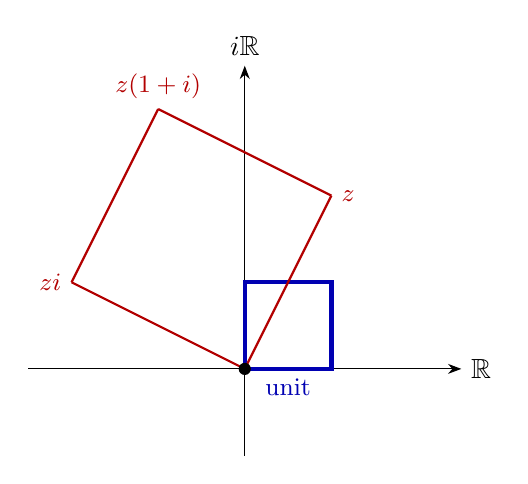
\begin{tikzpicture}[>=Stealth, scale=1.1]
  \draw[->] (-2.5,0) -- (2.5,0) node[right] {$\mathbb{R}$};
  \draw[->] (0,-1) -- (0,3.5) node[above] {$i\mathbb{R}$};

  % Blue unit square
  \draw[ultra thick, blue!70!black] (0,0) -- (1,0) -- (1,1) -- (0,1) -- (0,0);

  % Red transformed square
  \draw[thick, red!70!black] (0,0) -- (1,2) node[right] {\small $z$};
  \draw[thick, red!70!black] (0,0) -- (-2,1) node[left] {\small $zi$};
  \draw[thick, red!70!black] (-2,1) -- (-1,3) node[above] {\small $z(1+i)$};
  \draw[thick, red!70!black] (1,2) -- (-1,3);

  \fill (0,0) circle (2pt);
  \node[blue!70!black, below] at (0.5,0) {\small unit};
\end{tikzpicture}
\end{center}

\vfill

Here $z = 1 + 2i$. The blue $1 \times 1$ square is mapped to the red tilted square.

\end{frame}


\begin{frame}{Step 1: Rotate}

\begin{columns}
\column{0.5\textwidth}
\begin{center}
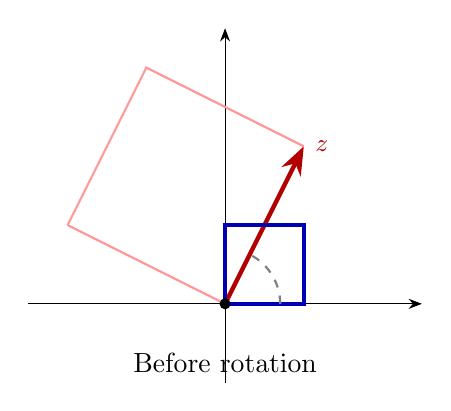
\begin{tikzpicture}[>=Stealth, scale=1.0]
  \draw[->] (-2.5,0) -- (2.5,0);
  \draw[->] (0,-1) -- (0,3.5);

  \draw[ultra thick, red!70!black, ->] (0,0) -- (1,2) node[right] {\small $z$};
  \draw[thick, red!40] (0,0) -- (-2,1);
  \draw[thick, red!40] (-2,1) -- (-1,3) -- (1,2);

  % Blue square (original)
  \draw[ultra thick, blue!70!black] (0,0) -- (1,0) -- (1,1) -- (0,1) -- (0,0);

  \draw[thick, gray, dashed] (0.7,0) arc[start angle=0, end angle=63.4, radius=0.7];

  \fill (0,0) circle (2pt);
  \node[below] at (0,-0.5) {Before rotation};
\end{tikzpicture}
\end{center}

\column{0.5\textwidth}
\begin{center}
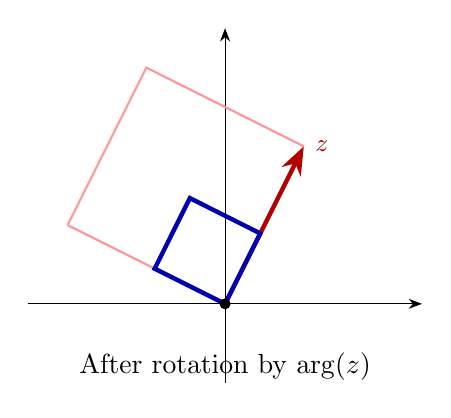
\begin{tikzpicture}[>=Stealth, scale=1.0]
  \draw[->] (-2.5,0) -- (2.5,0);
  \draw[->] (0,-1) -- (0,3.5);

  \draw[ultra thick, red!70!black, ->] (0,0) -- (1,2) node[right] {\small $z$};
  \draw[thick, red!40] (0,0) -- (-2,1);
  \draw[thick, red!40] (-2,1) -- (-1,3) -- (1,2);

  % Blue square (rotated but not scaled)
  \draw[ultra thick, blue!70!black] (0,0) -- (0.447,0.894) -- (-0.447,1.342) -- (-0.894,0.447) -- (0,0);

  \fill (0,0) circle (2pt);
  \node[below] at (0,-0.5) {After rotation by $\arg(z)$};
\end{tikzpicture}
\end{center}
\end{columns}

\vfill

\x{Rotate} the blue square by the angle $\arg(z) = \arctan \frac{b}{a}$.

\vfill

This is the angle between $z$ and the positive real axis.

\end{frame}


\begin{frame}{Step 2: Scale}

\begin{columns}
\column{0.5\textwidth}
\begin{center}
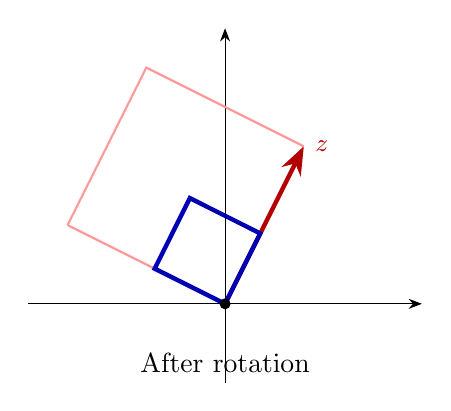
\begin{tikzpicture}[>=Stealth, scale=1.0]
  \draw[->] (-2.5,0) -- (2.5,0);
  \draw[->] (0,-1) -- (0,3.5);

  \draw[ultra thick, red!70!black, ->] (0,0) -- (1,2) node[right] {\small $z$};
  \draw[thick, red!40] (0,0) -- (-2,1);
  \draw[thick, red!40] (-2,1) -- (-1,3) -- (1,2);

  \draw[ultra thick, blue!70!black] (0,0) -- (0.447,0.894) -- (-0.447,1.342) -- (-0.894,0.447) -- (0,0);

  \fill (0,0) circle (2pt);
  \node[below] at (0,-0.5) {After rotation};
\end{tikzpicture}
\end{center}

\column{0.5\textwidth}
\begin{center}
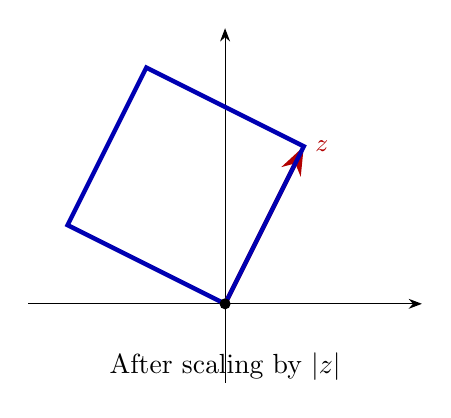
\begin{tikzpicture}[>=Stealth, scale=1.0]
  \draw[->] (-2.5,0) -- (2.5,0);
  \draw[->] (0,-1) -- (0,3.5);

  \draw[ultra thick, red!70!black, ->] (0,0) -- (1,2) node[right] {\small $z$};
  \draw[thick, red!70!black] (0,0) -- (-2,1);
  \draw[thick, red!70!black] (-2,1) -- (-1,3) -- (1,2);

  % Blue square stretched to match red
  \draw[ultra thick, blue!70!black] (0,0) -- (1,2) -- (-1,3) -- (-2,1) -- (0,0);

  \fill (0,0) circle (2pt);
  \node[below] at (0,-0.5) {After scaling by $|z|$};
\end{tikzpicture}
\end{center}
\end{columns}

\vfill

\x{Scale} by $|z| = \sqrt{a^2 + b^2}$, the \x{absolute value} of $z$.

\vfill

For $z = 1 + 2i$: $|z| = \sqrt{1^2 + 2^2} = \sqrt{5}$.

\end{frame}


\begin{frame}{Summary: Multiplication = Rotation + Scaling}

\begin{block}{Geometric meaning of complex multiplication}
Multiplying by $z = a + bi$:

\begin{enumerate}
\item \x{Rotate} by $\arg(z) = \arctan\frac{b}{a}$ \quad (the angle of $z$)
\item \x{Scale} by $|z| = \sqrt{a^2 + b^2}$ \quad (the length of $z$)
\end{enumerate}

\vfill

Equivalently: the unique transformation that sends $1 \mapsto z$.
\end{block}

\vfill\pause

\x{Special case:} Multiplying by $i$:
\begin{itemize}
\item $|i| = 1$ \quad (no scaling)
\item $\arg(i) = 90^{\circ}$ \quad (pure rotation)
\end{itemize}

\vfill

\x{This is why multiplication by $i$ is exactly $90^{\circ}$ rotation.}

\end{frame}


% ┌─────────────────────────────────────────────────────────────────────┐
% │ SECTION 5: POLAR FORM, DE MOIVRE & ROOTS OF UNITY                │
% │                                                                    │
% │ Legacy source: MANR.tex lines 203–262 + 8.0004.tex               │
% │ The polar form formalizes what §4 showed visually.                │
% │ De Moivre gives the power formula. Roots of unity are the first  │
% │ application: equally spaced points on the unit circle.            │
% └─────────────────────────────────────────────────────────────────────┘
\section{Polar Form, De Moivre \& Roots of Unity}


\begin{frame}{Polar Form}

From §4, every complex number $z = a + bi$ is determined by:
\begin{itemize}
\item its \x{absolute value} $|z| = \sqrt{a^2 + b^2}$ \quad (distance from origin)
\item its \x{argument} $\arg(z) = \arctan\frac{b}{a}$ \quad (angle from real axis)
\end{itemize}

\vfill

\begin{columns}
\column{0.45\textwidth}
\begin{center}
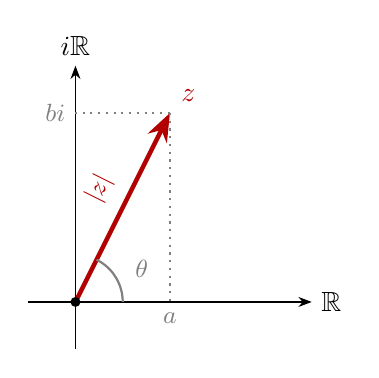
\begin{tikzpicture}[>=Stealth, scale=1.2]
  \draw[->] (-0.5,0) -- (2.5,0) node[right] {$\mathbb{R}$};
  \draw[->] (0,-0.5) -- (0,2.5) node[above] {$i\mathbb{R}$};

  \draw[ultra thick, red!70!black, ->] (0,0) coordinate (O) -- (1,2) coordinate (Z) node[above right] {$z$};
  \draw[thick, dotted, gray] (1,2) -- (1,0) node[below] {\small $a$};
  \draw[thick, dotted, gray] (1,2) -- (0,2) node[left] {\small $bi$};

  \draw[thick, gray] (0.5,0) arc[start angle=0, end angle=63.4, radius=0.5];
  \node[gray] at (0.7,0.35) {\small $\theta$};
  \node[red!70!black, rotate=63.4] at (0.25,1.2) {\small $|z|$};

  \fill (0,0) circle (1.5pt);
\end{tikzpicture}
\end{center}

\column{0.55\textwidth}

\x{Polar form:}
$$z = |z|(\cos\theta + i\sin\theta)$$

where $\theta = \arg(z)$.

\vfill

Real part: $a = |z|\cos\theta$

Imaginary part: $b = |z|\sin\theta$

\end{columns}

\end{frame}


\begin{frame}{Multiplication in Polar Form}

If $z_1 = |z_1|(\cos\theta_1 + i\sin\theta_1)$ and $z_2 = |z_2|(\cos\theta_2 + i\sin\theta_2)$, then:

\vfill

$$z_1 z_2 = |z_1||z_2|\bigl(\cos(\theta_1 + \theta_2) + i\sin(\theta_1 + \theta_2)\bigr)$$

\vfill\pause

\begin{block}{Two rules}
\x{Absolute values multiply:} $|z_1 z_2| = |z_1| \cdot |z_2|$

\vfill

\x{Arguments add:} $\arg(z_1 z_2) = \arg(z_1) + \arg(z_2)$
\end{block}

\vfill

This is the polar-form version of ``rotation + scaling.''

\end{frame}


\begin{frame}{De Moivre's Formula}

Applying the multiplication rule $n$ times:

$$z^n = |z|^n\bigl(\cos(n\theta) + i\sin(n\theta)\bigr)$$

\vfill\pause

\x{Special case:} If $|z| = 1$ (on the unit circle), then:

$$(\cos\theta + i\sin\theta)^n = \cos(n\theta) + i\sin(n\theta)$$

\vfill

\x{Raising to the $n$-th power = multiplying the angle by $n$.}

\end{frame}


\begin{frame}[shrink=3]{Roots of Unity}

\x{Question:} Which complex numbers satisfy $z^n = 1$?

\vfill\pause

By De Moivre: need $|z|^n = 1$ and $n\theta = 2\pi k$ for some integer $k$.

So $|z| = 1$ and $\theta = \frac{2\pi k}{n}$, giving $n$ equally spaced points on the unit circle.

\vfill

\begin{columns}
\column{0.5\textwidth}
\begin{center}
\textbf{3rd roots of unity}

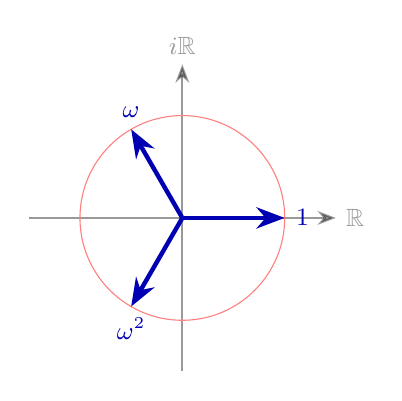
\begin{tikzpicture}[>=Stealth, scale=1.3]
  \draw[->,thick,opacity=0.4] (-1.5,0) -- (1.5,0) node[right] {\small $\mathbb{R}$};
  \draw[->,thick,opacity=0.4] (0,-1.5) -- (0,1.5) node[above] {\small $i\mathbb{R}$};
  \draw[red!50] (0,0) circle[radius=1];
  \draw[->,blue!70!black,ultra thick] (0,0) -- (1,0) node[right] {\small $1$};
  \draw[->,blue!70!black,ultra thick] (0,0) -- (-0.5,0.866) node[above] {\small $\omega$};
  \draw[->,blue!70!black,ultra thick] (0,0) -- (-0.5,-0.866) node[below] {\small $\omega^2$};
\end{tikzpicture}

$1 + \omega + \omega^2 = 0$
\end{center}

\column{0.5\textwidth}
\begin{center}
\textbf{4th roots of unity}

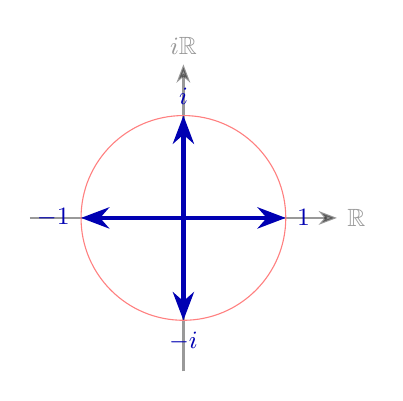
\begin{tikzpicture}[>=Stealth, scale=1.3]
  \draw[->,thick,opacity=0.4] (-1.5,0) -- (1.5,0) node[right] {\small $\mathbb{R}$};
  \draw[->,thick,opacity=0.4] (0,-1.5) -- (0,1.5) node[above] {\small $i\mathbb{R}$};
  \draw[red!50] (0,0) circle[radius=1];
  \draw[->,blue!70!black,ultra thick] (0,0) -- (1,0) node[right] {\small $1$};
  \draw[->,blue!70!black,ultra thick] (0,0) -- (0,1) node[above] {\small $i$};
  \draw[->,blue!70!black,ultra thick] (0,0) -- (-1,0) node[left] {\small $-1$};
  \draw[->,blue!70!black,ultra thick] (0,0) -- (0,-1) node[below] {\small $-i$};
\end{tikzpicture}

$1 + i + i^2 + i^3 = 0$
\end{center}
\end{columns}

\end{frame}


% ┌─────────────────────────────────────────────────────────────────────┐
% │ SECTION 6: CONJUGATE, DIVISION & THE PHILOSOPHY OF SYMMETRY       │
% │                                                                    │
% │ THE MACRO DESIGN: SYMMETRY AS A DEEP PRINCIPLE                    │
% │                                                                    │
% │ This is a MUST section per the user. Conjugation is not just a    │
% │ formula — it is the fundamental symmetry of C over R. The         │
% │ Steiner tree (four villages) example from MAN2.tex makes this     │
% │ concrete: symmetric problem → asymmetric solution → conjugation   │
% │ produces another solution → sum recovers symmetry.                │
% │                                                                    │
% │ Legacy source: MANR.tex lines 295–335 + MAN2.tex lines 325–400.  │
% └─────────────────────────────────────────────────────────────────────┘
\section[Conjugate, Division \& Symmetry]{Conjugate, Division \& The Philosophy of Symmetry}


\begin{frame}[shrink=5]{Conjugate}

For $z = a + bi$, the \x{conjugate} is:

$$\bar{z} := a - bi$$

\vfill

\begin{center}
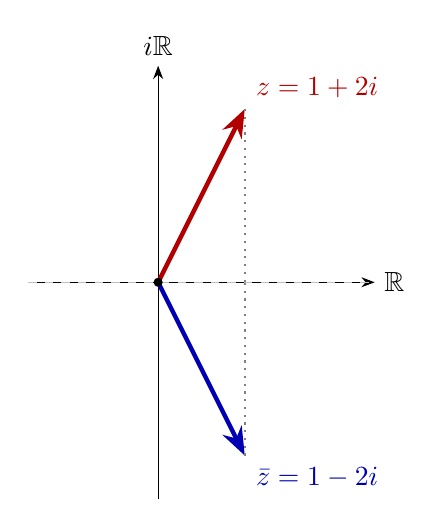
\begin{tikzpicture}[>=Stealth, scale=1.1]
  \draw[->] (-1.5,0) -- (2.5,0) node[right] {$\mathbb{R}$};
  \draw[->] (0,-2.5) -- (0,2.5) node[above] {$i\mathbb{R}$};

  \draw[ultra thick, red!70!black, ->] (0,0) -- (1,2) node[above right] {$z = 1 + 2i$};
  \draw[ultra thick, blue!70!black, ->] (0,0) -- (1,-2) node[below right] {$\bar{z} = 1 - 2i$};

  \draw[thick, dotted, gray] (1,2) -- (1,0);
  \draw[thick, dotted, gray] (1,-2) -- (1,0);
  \draw[dashed, gray!50] (-1.5,0) -- (2.5,0);

  \fill (0,0) circle (1.5pt);
\end{tikzpicture}
\end{center}

\vfill

\x{Reflection} across the real axis. Same real part, opposite imaginary part.

\end{frame}


\begin{frame}{Properties of Conjugation}

\x{Key identity:}
$$z\bar{z} = (a+bi)(a-bi) = a^2 + b^2 = |z|^2 \qquad \text{(always real, always $\geq 0$)}$$

\vfill\pause

\x{Extracting parts:}
$$\text{Real part: } a = \frac{z + \bar{z}}{2}, \qquad \text{Imaginary part: } b = \frac{z - \bar{z}}{2i}$$

\vfill\pause

\x{Division:} To compute $\frac{3+4i}{2+i}$, multiply top and bottom by the conjugate of the denominator:

$$\frac{3+4i}{2+i} = \frac{(3+4i)\overline{(2+i)}}{(2+i)\overline{(2+i)}} = \frac{(3+4i)(2-i)}{|2+i|^2} = \frac{10 + 5i}{5} = 2 + i$$

\end{frame}


\begin{frame}{What is Symmetry?}

In mathematics, \x{symmetry} means \x{invariant under a certain action}.

\vfill

The action on $\mathbb{C}$: \x{conjugation} $z \mapsto \bar{z}$.

\vfill\pause

Which numbers are \x{symmetric} (invariant)?

$$\bar{z} = z \quad\iff\quad a - bi = a + bi \quad\iff\quad b = 0 \quad\iff\quad z \in \mathbb{R}$$

\vfill

The \x{real numbers} are exactly the symmetric elements of $\mathbb{C}$ under conjugation.

\vfill\pause

\begin{block}{The Symmetry Principle}
If a \x{symmetric system} produces an \x{asymmetric result}, then performing the symmetry action on that result produces \x{another valid result}.

\vfill

Collecting all such results \x{recovers the symmetry}.
\end{block}

\end{frame}


\begin{frame}[shrink=5]{Example: Four Villages}

Four villages at the vertices of a square. The system is \x{symmetric under $90^{\circ}$ rotation}.

\vfill

\begin{center}
\begin{tikzpicture}[scale=0.7]
  \draw[fill=black] (0,0) circle(0.12) node[below left] {A};
  \draw[fill=black] (4,0) circle(0.12) node[below right] {B};
  \draw[fill=black] (4,4) circle(0.12) node[above right] {C};
  \draw[fill=black] (0,4) circle(0.12) node[above left] {D};
\end{tikzpicture}
\end{center}

\vfill

\x{Problem:} Find the \x{shortest road network} connecting all four villages.

\end{frame}


\begin{frame}[shrink=3]{Asymmetric Solution}

\begin{columns}
\column{0.45\textwidth}
\begin{center}
\textbf{Solution 1}

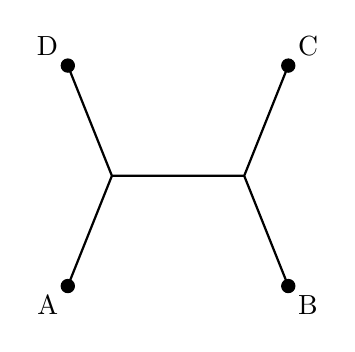
\begin{tikzpicture}[scale=0.7]
  \draw[thick] (0,0)--(0.8,2)--(3.2,2)--(4,0) (0,4)--(0.8,2) (4,4)--(3.2,2);
  \draw[fill=black] (0,0) circle(0.12) node[below left] {A};
  \draw[fill=black] (4,0) circle(0.12) node[below right] {B};
  \draw[fill=black] (4,4) circle(0.12) node[above right] {C};
  \draw[fill=black] (0,4) circle(0.12) node[above left] {D};
\end{tikzpicture}
\end{center}

\column{0.55\textwidth}

This shortest road is \x{asymmetric} --- it is NOT invariant under $90^{\circ}$ rotation.

\vfill\pause

But the problem IS symmetric!

\vfill

So the symmetry action ($90^{\circ}$ rotation) applied to this solution must give \x{another valid shortest road}.

\end{columns}

\vfill\pause

\begin{columns}
\column{0.45\textwidth}
\begin{center}
\textbf{Solution 2} (rotated by $90^{\circ}$)

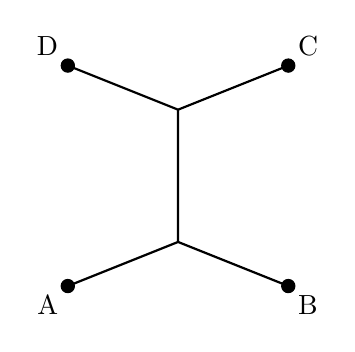
\begin{tikzpicture}[scale=0.7]
  \draw[thick] (0,0)--(2,0.8)--(2,3.2)--(0,4) (4,0)--(2,0.8) (4,4)--(2,3.2);
  \draw[fill=black] (0,0) circle(0.12) node[below left] {A};
  \draw[fill=black] (4,0) circle(0.12) node[below right] {B};
  \draw[fill=black] (4,4) circle(0.12) node[above right] {C};
  \draw[fill=black] (0,4) circle(0.12) node[above left] {D};
\end{tikzpicture}
\end{center}

\column{0.55\textwidth}

Also a shortest road. Also asymmetric.

\end{columns}

\end{frame}


\begin{frame}{Symmetry Recovered}

Overlay \x{both} solutions:

\vfill

\begin{center}
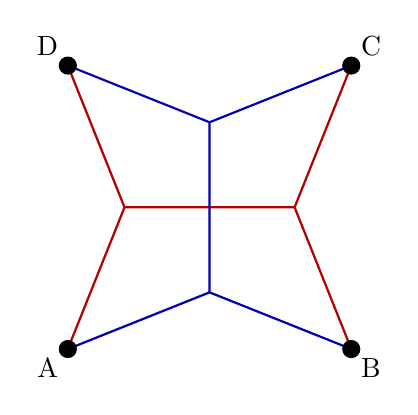
\begin{tikzpicture}[scale=0.9]
  \draw[thick, red!70!black] (0,0)--(0.8,2)--(3.2,2)--(4,0) (0,4)--(0.8,2) (4,4)--(3.2,2);
  \draw[thick, blue!70!black] (0,0)--(2,0.8)--(2,3.2)--(0,4) (4,0)--(2,0.8) (4,4)--(2,3.2);
  \draw[fill=black] (0,0) circle(0.12) node[below left] {A};
  \draw[fill=black] (4,0) circle(0.12) node[below right] {B};
  \draw[fill=black] (4,4) circle(0.12) node[above right] {C};
  \draw[fill=black] (0,4) circle(0.12) node[above left] {D};
\end{tikzpicture}
\end{center}

\vfill

The combined figure \x{is symmetric} under $90^{\circ}$ rotation!

\vfill\pause

\x{Individual solutions break the symmetry. The collection of all solutions recovers it.}

\end{frame}


\begin{frame}{Symmetry Principle Applied to Complex Numbers}

\x{A real polynomial is a symmetric system} --- it is invariant under conjugation.

\vfill

If a real polynomial has a complex root $z$, then $\bar{z}$ must also be a root.

\vfill\pause

$$t^2 - 2t + 5 = 0 \quad\implies\quad t = 1 + 2i \;\;\text{and}\;\; t = \overline{1+2i} = 1 - 2i$$

\vfill\pause

\begin{block}{Complex roots of real polynomials come in conjugate pairs}
If $p(t)$ has real coefficients and $p(z) = 0$, then $p(\bar{z}) = 0$.
\end{block}

\vfill

This is the \x{same philosophy} as the four villages: the real polynomial is the symmetric problem, the complex root is the asymmetric solution, and conjugation produces the partner.

\end{frame}


\begin{frame}{Symmetry of Eigenstructure}

If $A$ is a \x{real matrix}, then $\det(tI - A)$ is a \x{real polynomial}.

\vfill

So eigenvalues come in conjugate pairs:

$$\text{If } \lambda = a + bi \text{ is an eigenvalue, so is } \bar{\lambda} = a - bi.$$

\vfill\pause

And the \x{eigenvectors} also come in conjugate pairs:

$$\text{If } A\mathbf{v} = \lambda \mathbf{v}, \text{ then } A\bar{\mathbf{v}} = \bar{\lambda}\bar{\mathbf{v}}.$$

\vfill\pause

\begin{block}{The symmetry principle applies to the entire eigenstructure}
For real matrices: eigenvalues, eigenvectors, and spectral projections all respect conjugation.

\vfill

This is not a coincidence --- it is a direct consequence of the symmetry of real coefficients under conjugation.
\end{block}

\end{frame}


% ┌─────────────────────────────────────────────────────────────────────┐
% │ SECTION 7: THE FUNDAMENTAL THEOREM & COMPLEX EIGENVALUES          │
% │                                                                    │
% │ THE MACRO DESIGN: THE PAYOFF — PIPELINE RESTORED                  │
% │                                                                    │
% │ We return to the problem from §1. The FTA guarantees every        │
% │ polynomial factors over C. The pipeline works again. We show      │
% │ the rotation matrix now has eigenvalues ±i, and a second example  │
% │ with eigenvalues 1±2i. End by clarifying: this is a PARTIAL fix. │
% │ Repeated factors in the minimal polynomial = JCF (self-study).   │
% └─────────────────────────────────────────────────────────────────────┘
\section[Fundamental Theorem \& Eigenvalues]{The Fundamental Theorem \& Complex Eigenvalues}


\begin{frame}{Fundamental Theorem of Algebra}

\begin{thm}[Fundamental Theorem of Algebra]
Every degree-$n$ polynomial with complex coefficients has exactly $n$ roots in $\mathbb{C}$ (counted with multiplicity):

$$p(t) = (t - z_1)(t - z_2)\cdots(t - z_n), \qquad z_i \in \mathbb{C}$$
\end{thm}

\vfill\pause

\x{Every polynomial factors into linear factors over $\mathbb{C}$.}

\vfill

No exceptions. No irreducible quadratics. No polynomials that ``don't factor.''

\end{frame}


\begin{frame}{The Pipeline Works Again}

For \x{any} $n \times n$ matrix $A$:

\vfill

$\det(tI - A)$ is degree $n$ \quad$\implies$\quad it has $n$ complex roots.

\vfill

\x{Every matrix has eigenvalues over $\mathbb{C}$.}

\vfill\pause

\begin{center}
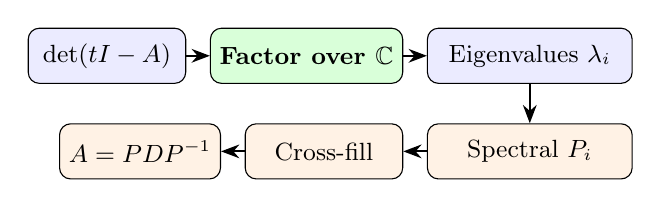
\begin{tikzpicture}[>=Stealth, node distance=0.3cm, every node/.style={font=\small}]
  \node[draw, rounded corners, fill=blue!8, minimum width=2.0cm, minimum height=0.7cm] (det) {$\det(tI - A)$};
  \node[right=of det, draw, rounded corners, fill=green!15, minimum width=1.6cm, minimum height=0.7cm] (fac) {\x{Factor over $\mathbb{C}$}};
  \node[right=of fac, draw, rounded corners, fill=blue!8, minimum width=2.6cm, minimum height=0.7cm] (eig) {Eigenvalues $\lambda_i$};

  \node[below=0.5cm of eig, draw, rounded corners, fill=orange!10, minimum width=2.6cm, minimum height=0.7cm] (spec) {Spectral $P_i$};
  \node[left=of spec, draw, rounded corners, fill=orange!10, minimum width=2.0cm, minimum height=0.7cm] (cross) {Cross-fill};
  \node[left=of cross, draw, rounded corners, fill=orange!10, minimum width=2.0cm, minimum height=0.7cm] (diag) {$A = PDP^{-1}$};

  \draw[->, thick] (det) -- (fac);
  \draw[->, thick] (fac) -- (eig);
  \draw[->, thick] (eig) -- (spec);
  \draw[->, thick] (spec) -- (cross);
  \draw[->, thick] (cross) -- (diag);
\end{tikzpicture}
\end{center}

\vfill

The ``Factor'' step \x{never fails} over $\mathbb{C}$. The pipeline runs for all matrices with distinct eigenvalues.

\end{frame}


\begin{frame}[shrink=5]{Example 1: The Rotation Matrix Revisited}

$$R = \begin{pmatrix} 0 & -1 \\ 1 & 0 \end{pmatrix}, \qquad \det(tI - R) = t^2 + 1$$

\vfill

Over $\mathbb{R}$: \x{can't factor}. Pipeline stops.

\vfill\pause

Over $\mathbb{C}$:

$$t^2 + 1 = (t - i)(t + i)$$

Eigenvalues: $\lambda_1 = i$, $\lambda_2 = -i$. \quad \x{Conjugate pair}, as the symmetry principle predicts.

\vfill\pause

Two distinct eigenvalues $\implies$ the pipeline works:

$$P_i = \frac{R - (-i)I}{i - (-i)} = \frac{R + iI}{2i}, \qquad P_{-i} = \frac{R - iI}{-2i}$$

$$R = i \cdot P_i + (-i) \cdot P_{-i}$$

\end{frame}


\begin{frame}{Example 2: Eigenvalues $1 \pm 2i$}

$$A = \begin{pmatrix} 1 & 2 \\ -2 & 1 \end{pmatrix}, \qquad \det(tI - A) = t^2 - 2t + 5$$

\vfill

Over $\mathbb{C}$:

$$t^2 - 2t + 5 = \bigl(t - (1+2i)\bigr)\bigl(t - (1-2i)\bigr)$$

\vfill\pause

Eigenvalues: $1 + 2i$ and $1 - 2i$. \quad Conjugate pair.

\vfill

Eigenvectors: $\begin{pmatrix}1\\i\end{pmatrix}$ for $\lambda = 1+2i$, \quad $\begin{pmatrix}1\\-i\end{pmatrix}$ for $\lambda = 1-2i$.

\vfill

Conjugate pair of eigenvectors for conjugate pair of eigenvalues.

\vfill\pause

\x{The symmetry principle in action}: real matrix $\implies$ everything conjugates.

\end{frame}


\begin{frame}{What We Have Achieved}

\begin{block}{Restriction (a): Resolved}
Over $\mathbb{C}$, every polynomial factors into linear factors.

\vfill

Our pipeline works for all matrices whose minimal polynomial has \x{distinct roots} --- regardless of whether eigenvalues are real or complex.
\end{block}

\vfill\pause

\begin{block}{Restriction (b): Still open}
Repeated factors in the minimal polynomial $\implies$ Lagrange interpolation fails (observation points collapse).

\vfill

This requires \x{Jordan Canonical Form} --- self-study material.

\vfill

Complex numbers do not solve this.
\end{block}

\end{frame}


% ┌─────────────────────────────────────────────────────────────────────┐
% │ SECTION 8: PREVIEW                                                │
% │                                                                    │
% │ Bridge to the next lecture: exponential functions.                 │
% │ Now that eigenvalues can be complex, what does e^lambda mean?     │
% └─────────────────────────────────────────────────────────────────────┘
\section{Preview}


\begin{frame}{What We Have Gained}

Every matrix with distinct eigenvalues (over $\mathbb{C}$) is diagonalizable:

$$A = PDP^{-1}$$

\vfill

\x{Spectral decomposition}, \x{value tables}, \x{$A^n$} --- all work with complex eigenvalues.

\vfill

The rotation matrix $R$ with eigenvalues $\pm i$, the matrix $A$ with eigenvalues $1 \pm 2i$ --- our full machinery applies.

\end{frame}


\begin{frame}{Next Lecture: The Exponential Function}

We can compute $A^n = PD^nP^{-1}$. But what about $e^A$?

\vfill\pause

If $A = PDP^{-1}$, then we would want:

$$e^A = Pe^DP^{-1} = P\begin{pmatrix}e^{\lambda_1} & \\ & e^{\lambda_2}\end{pmatrix}P^{-1}$$

\vfill\pause

\x{The question:} What does $e^{\lambda}$ mean when $\lambda$ is \x{complex}?

\vfill

What is $e^{i\theta}$? What is $e^{1+2i}$?

\vfill\pause

\x{Next lecture:} We will discover that $e^{i\theta} = \cos\theta + i\sin\theta$, and use this to solve systems of differential equations $\mathbf{y}' = A\mathbf{y}$.

\end{frame}


\end{document}
